\documentclass{article}
\usepackage{amsmath, enumitem}
\usepackage{graphicx}
\usepackage{booktabs}
\usepackage{tabularx}
\usepackage[margin=1in]{geometry}
\usepackage{float}
\restylefloat{table}
\usepackage{placeins}



\begin{document}

\title{Econ 741 Homework 3}
\author{John Appert, Randall Chicolla, Andrea Franz}
\maketitle

\section{Question 1:  Polynomials (Stata)}
Let’s see how income varies with age. First construct your sample. We will want to
study individuals who are (inclusively) between 16 and 65 years of age, have positive earnings, and worked more than 1000 hours in a year. Pick a polynomial specification (of age) to run.

\begin{enumerate}[label=\alph*]
\item Present the results from your regression.  (5 points)

\item Explain why you picked the specification you did.  (6 points)

\item  Give the marginal effect and the average of the marginal effects.  (4 points)

\item  Discuss the significance of your polynomial overall as well as the individual terms.  (4 points)

\end{enumerate}

\section{Question 2:  Indicator Variables and Interactions  (Stata)}
Let’s now see how earnings varies with marriage. Use the marst variable to create
three indicator variables for whether people are a) never married b) currently married c) formerly married.

\begin{enumerate}[label=\alph*]
\item  Put all three indicator variables into your model. Discuss the results. (6 points)

\item Run a model that will test whether or not married people see their wages go up
more quickly with age than people who were never married. Discuss the results.
(8 points)

\end{enumerate}

\section{Question 3:  Functional Form (Stata)}
Construct a variable that is years of education. Report and interpret (in one sentence each) the following coefficients with a model of earnings on education:

\begin{enumerate}[label=\alph*]

\item Linear-Linear (4 points)

In the linear-linear model $\beta_0$ is -23558 and $\beta_1$ is 4759.  This implies that every year of additional education is worth 4800 dollars in increased wages.  However, there is obviously a problem with this model as at no education it predicts negative wages.

\item Log-Linear (4 points)

In the Log linear model $\beta_0$ is 0.87 and $\beta_1$ is 0.11.  This implies that every additional year of education increases earnings by 11 percent.

\item Linear-Log (4 points)

In the linear log model $\beta_0$ is -159301.4  and $\beta_1$ is 76774.66.  ???

\item Log-Log (4 points)

In the log log mode $\beta_0$ is  5.544492 and $\beta_1$ is  1.771558.  This implies that the elasticity of wages to education is 1.77 and that at no education wages are expected to be roughly 244 dollars.

\end{enumerate}

\section{Question 4:  Heteroskedasticity (Stata and R)}

\begin{enumerate}[label=\alph*]

\item Is there evidence of heteroskedasticity based on age? Show me in a picture.
Discuss. (12 points)\\

Yes.  If there were no heteroskedasticity in the data the residuals plotted agains the independent variable would be random.  In the figure below we see that there is an upward curve in the data.  It is certainly not random.  Therefore the data shows clear heteroskedasticity.


\begin{figure}[ht!]
\centering
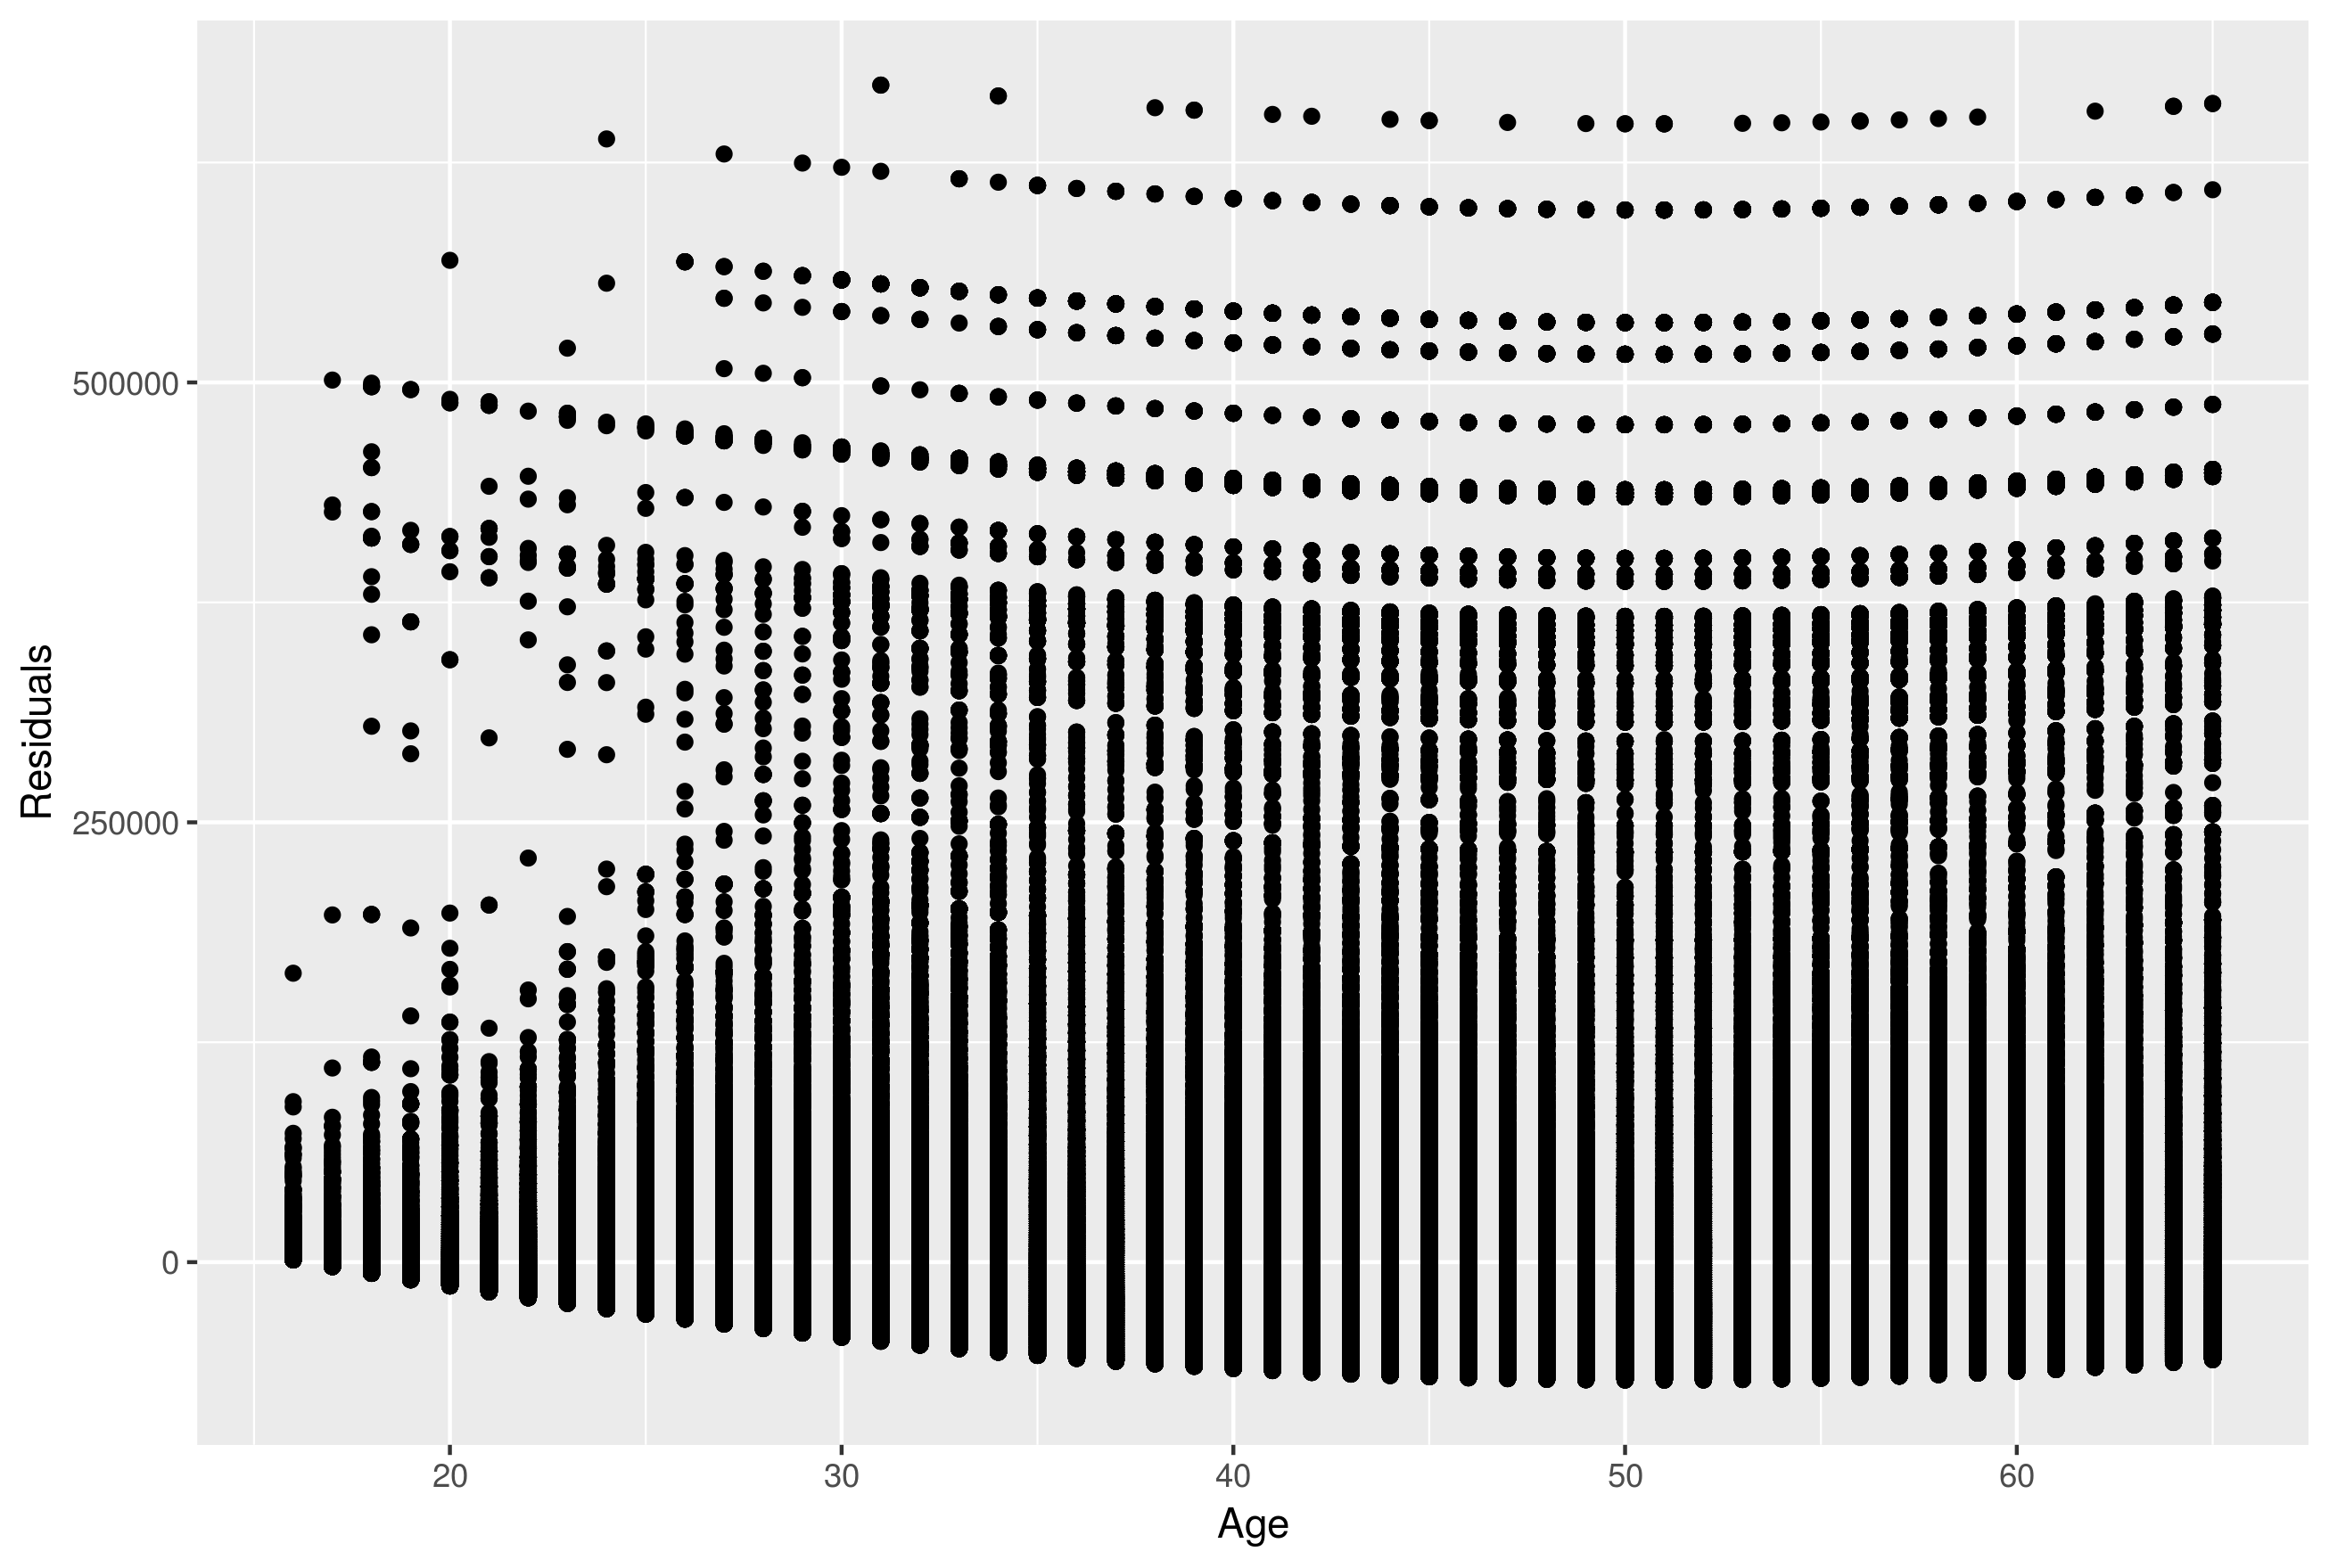
\includegraphics[width=90mm]{residuals.png}
\caption{Residuals vs Age \label{overflow}}
\end{figure}


\item Obtain robust standard errors in R and Stata. (18 points)

The values of the robust standard errors found in R were as follows:\\
With no adjustment for degrees of freedom:

Age:  23.6251\\
Age2:  0.3024647\\
Cons:  399.5719148\\

We adjusted these values for the degrees of freedom using:

$ N/(N-k)$

Age:  23.625128\\
Age2:  0.302465 \\
Cons:  399.572365\\

Using Stata we found the following values for robust standard errors:

Age:  23.62513\\
Age2:  0.302465 \\
Cons:  399.5724\\

\end{enumerate}
\end{document}

